% options:
% thesis=B bachelor's thesis
% thesis=M master's thesis
% czech thesis in Czech language
% slovak thesis in Slovak language
% english thesis in English language
% hidelinks remove colour boxes around hyperlinks

\documentclass[thesis=B,czech]{FITthesis}[2012/06/26]

\usepackage[utf8]{inputenc} % LaTeX source encoded as UTF-8

\usepackage{graphicx} %graphics files inclusion
% \usepackage{amsmath} %advanced maths
% \usepackage{amssymb} %additional math symbols

\usepackage{dirtree} %directory tree visualisation

% % list of acronyms


\usepackage[acronym,nonumberlist,toc,numberedsection=autolabel]{glossaries}
\iflanguage{czech}{\renewcommand*{\acronymname}{Seznam pou{\v z}it{\' y}ch zkratek}}{}
\makeglossaries

\usepackage{todonotes}
\usepackage{enumitem}
\usepackage{hyperref}
\usepackage{tabularx}
\usepackage{spverbatim}
\usepackage{listings}
\usepackage{caption}

\DeclareCaptionFont{white}{\color{white}}
\DeclareCaptionFormat{listing}{\colorbox{gray}{\parbox{\textwidth}{#1#2#3}}}
\captionsetup[lstlisting]{format=listing,labelfont=white,textfont=white}

\newcommand{\tg}{\mathop{\mathrm{tg}}} %cesky tangens
\newcommand{\cotg}{\mathop{\mathrm{cotg}}} %cesky cotangens

\newcommand{\GTD}{\textit{GTD }}
\newcommand{\textctandit}[1]{\textit{\uv{#1}}}

% % % % % % % % % % % % % % % % % % % % % % % % % % % % % % 
% ODTUD DAL VSE ZMENTE
% % % % % % % % % % % % % % % % % % % % % % % % % % % % % % 

\department{Katedra softwarového inženýrství}
\title{GTD - Mít vše hotovo}
\authorGN{Michal} %(křestní) jméno (jména) autora
\authorFN{Sláma} %příjmení autora
\authorWithDegrees{Michal Sláma} %jméno autora včetně současných akademických titulů
\supervisor{Ing. Jiří Mlejnek}
\acknowledgements{Děkuji vedoucímu své práce za hodnotné rady a své rodině za podporu při vytváření této práce.}
\abstractCS{Má bakalářská práce se zabývá návrhem a realizací systému osobního plánování na základě metodiky \cite{gtd}. V této práci vytvořím aplikaci pro centrální uložení dat dostupné přes REST API a mobilní aplikaci pro OS Android napojenou na zmíněné API a poskytují funkce osobního plánování. Zároveň umožním uživateli publikovat své úkoly na Facebook a do Google kalendáře.}
\abstractEN{Sem doplňte ekvivalent abstraktu Vaší práce v~angličtině.}
\placeForDeclarationOfAuthenticity{V~Praze}
\declarationOfAuthenticityOption{4} %volba Prohlášení (číslo 1-6)
\keywordsCS{webová aplikace, mobilní aplikace, osobní plánování, spring, android, REST API, Facebook, Google kalendář}
\keywordsEN{web application, mobile appliaction, personal planning, spring, android, REST API, Facebook, Google Calendar}

\lstset{
	basicstyle=\footnotesize\ttfamily,
	numberstyle=\tiny,
	numbersep=5pt,
	tabsize=2,
	extendedchars=true,
	breaklines=true,
	keywordstyle=\color{red},
	frame=b,         
	stringstyle=\color{white}\ttfamily,
	showspaces=false, 
	showtabs=false,  
	xleftmargin=17pt,
	framexleftmargin=17pt,
	framexrightmargin=5pt,
	framexbottommargin=4pt,
	showstringspaces=false, 
	breakatwhitespace=true,
	commentstyle=\color{pgreen},
	keywordstyle=\color{pblue},
	stringstyle=\color{pred}    
}
\lstloadlanguages{Java}

\begin{document}
 

\newacronym{CVUT}{{\v C}VUT}{{\v C}esk{\' e} vysok{\' e} u{\v c}en{\' i} technick{\' e} v Praze}
\newacronym{FIT}{FIT}{Fakulta informa{\v c}n{\' i}ch technologi{\' i}}
\newacronym{ws}{WS}{Web service}
\newacronym{api}{API}{Application Programming Interface}
\newacronym{os}{OS}{Operating system}
\newacronym{rest}{REST}{Representational State Transfer}
\newacronym{soap}{SOAP}{Simple Object Access protocol}
\newacronym{http}{HTTP}{Hypertext Transfer Protocol}
\newacronym{wsdl}{WSDL}{Web Services Description Language}
\newacronym{crud}{CRUD}{create-read-update-delete operations}
\newacronym{uri}{URI}{Uniform Resource Identifier}
\newacronym{wadl}{WADL}{Uniform Resource Identifier}
\newacronym{raml}{RAML}{RESTful API Modeling}
\newacronym{yaml}{YAML}{Ain’t Markup Language}
\newacronym{xml}{XML}{Extensible Markup Language}
\newacronym{json}{JSON}{JavaScript Object Notation}
\newacronym{orm}{ORM}{Object-relational mapping}
\newacronym{sdk}{SDK}{Software development kit}

\todototoc
\listoftodos


\todo{Co je obsaženo v práci, nikoliv na čem budu dělat}

\begin{introduction}
\begin{center}
\textit{\uv{Ze všeho nejvíce požírá čas a energii neustále neproduktivní přemýšlení o věcech, které musíme udělat.}}\\
Kerry Glesson
\end{center}

V současném informačním věku naše práce přestává být fyzickou. Práce už není ohraničena jasnými hranicemi a existuje velké množství informačních zdrojů použitelný pro její zpracování. Řešitel je tím vystaven tlaku nejasného zadání i rozsahu a musí si sám určit cíle své práce.

Naše mysl nejasné nepřijímá, jakékoliv takové úkoly nám neustále připomíná, vyžaduje se jejich řešení a znemožňuje nám tím koncentraci. Potřebujeme nový přístup. Přístup, abychom naši mysl dokázali přesvědčit, že máme vše jasné a právě teď se můžeme koncentrovat pouze na aktuální úkol.

Jedním z takových přístupu je metodika vytvořená Davidem Allenem \GTD\cite{gtd}. Jeho motto \textit{\uv{Jak zvládnout práci i život a cítit se při tom dobře}} je mým kýženým životním cílem.

Moje práce se zabývá návrhem a implementací informačního systému pro osobní plánování založeném na metodice GTD. Provedu analýzu samotné metodiky, navrhnu vhodnou infrastrukturu splňující potřebná kritéria \GTD\cite{gtd}, implementuji aplikaci pro centrální uložení dat a mobilní aplikaci pro uživatele.    

	
\end{introduction}

\chapter{Cíl práce}

První cílem mé práce je analyzovat metodiku \GTD\cite{gtd}. Prozkoumám existující implementace osobního plánování podporující \GTD\cite{gtd}. Navrhnu vlastní informační systém.

Vytvořím aplikaci poskytující \acrshort{ws} pro centrální uložení dat. Vyberu nejvhodnější typ webových služeb. Pro tuto aplikaci najdu potřebný hosting a na něm provedu konfiguraci aplikačního a databázového serveru.

Vytvořím mobilní aplikaci pro Android využívající \acrshort{ws} služeb předešlé aplikace. Aplikace umožní uživateli správu jeho osobního plánování.

Dnešní internetový svět je propojen skrze sociálních sítě. Proto umožním uživateli publikovat své úkoly do sítí \textit{Facebooku} a \textit{Google kalendáře}.K tomu nastuduji potřebné specifikace poskytovaných \acrshort{api}  

Mým cílem není vytvoření odladěné aplikace, ale získání know-how s vývojem takového systému.
  
\chapter{Analýza metodiky \GTD}

V této kapitole se zabývám analýzou metodiky \GTD, hledám její základní stavební prvky a její přínos pro osobní plánování. Definuji důležité pojmy a postupy pro využití v dalším návrhu aplikace. 
Dále srovnávám existující implementace osobního plánování a hledám jejich výhody, kterými podporují kvalitnější a přehlednější osobní plánování.
Na závěr spojuji výsledky obou předchozích bodů a navrhuji základní strukturu a funkce budoucí aplikace.

\section{Metodika GTD - Mít vše hotovo}

Kniha \GTD\cite{gtd} vznikla v roce 2001 a jejím autorem je David Allen. Samotná metodika nepředstavuje jasné řešení, podle kterého se můžeme okamžitě začít řídit a změníme tím svůj život. Snaží se vysvětlit obecné zákonitosti lidské mysli a najít takových způsob plánování, který s ní bude v souladu.\\


Pojďme se na metodiku podívat podrobněji.

\subsection{Změna práce}

Naše práce přestává být fyzikou a přesunuje se do roviny sběru informací, jejich zpracování a vytvoření závěrů. Zároveň nejsme schopni jednoznačně určit prioritu, protože ta se stává proměnnou závislou na mnoha vnějších i vnitřních faktorech. Naše práce přestává mít jasné hranice, které naše mysl potřebuje. Bez jasných hranic nám mysl bude takové věci neustále sama připomínat a vyžadovat se o jejich řešení. Paradoxem je, že naše mysl v tomto ohledu nejedná rozumně a připomíná nám naše nedořešené věci bez ohledu na vhodnost situace. Při takovém stavu si říkáme \textit{\uv{memohu se soustředit}}, mysl nám ruší naši vlastní koncentraci. A koncentrace je nutnou podmínkou pro vysokou výkonnost a my potřebujeme aktuálnímu úkolu věnovat 100\% pozornosti.

Jak toho ale dosáhnout? Potřebujeme naši mysl přesvědčit, že o všech úkolech víme, jsou zaznamenány mimo ní, víme přesně co máme dělat a není riziko zapomenutí.

\subsection{Produktivita}
\begin{center}
\textctandit{Ve znalostní práci není úkol dán, je třeba jej určit. Jaký je očekávaný výsledek práce? Je klíčovou otázkou pro produktivitu znalostních pracovníků. Je to otázka, která si žádá riskantního rozhodnutí. Obvykle na ni neexistuje správná odpověď, místo ní jsou tu možnosti. A má-li být dosaženo produktivity, je třeba jasně specifikovat očekávané výsledky.}\\
Petr Ducken\cite{gtd}
\end{center}

Mysl potřebuje jasný cíl, aby mohla udržet potřebné soustředění, nepřemohla ji únava a dokázala rozlišit důležité informace pro zapamatování.\\
\newline
\textit{Co udělat při zpracování úkolu:}
\begin{enumerate}[nosep]
	\item vyjasnit si požadovaný výsledek
	\item mít jasno o dalším kroku
	\item uložit si úkol do důvěryhodného systému
\end{enumerate}
\vspace*{1\baselineskip}
Začít je třeba od nezákladnější věcí. To nám pomůže zvládnout a odpoutat se od každodenních závazků a poté se můžeme lépe soustředit na větší projekty a vize. Při zpracování potřebujeme využít kontroly ve dvou rovinách: horizontální a vertikální. V horizontální přemýšlíme, co všechno potřebujeme udělat. Ve vertikální řešíme konkrétní věc a co je potřeba vykonat k jejímu splnění.\\ 
\newline
Typický horizontální postup:
\begin{enumerate}[nosep]
\item sběr věcí, které si získaly naší pozornost
\item hodnotíme jejich význam a kroky k jejich splnění
\item uspořádáme si výsledky
\item máme je v plánu a hledáme vhodný čas k provedení
\item provedeme
\end{enumerate}
\vspace*{1\baselineskip}
\subsubsection{Sběr věcí}
Pozornost si získávají věci u kterých si řekneme \textctandit{měl bych}, \textctandit{potřebuji}, \textctandit{musím}. Je potřeba sesbírat všechny věci a žádnou nelze vynechat. Pro naši mysl je důležitým slovem \textctandit{všechno} a nesmí vzniknout jakákoliv pochybnost. V tuto chvíli ještě nepotřebujeme pouze jedno místo uložení, protože spojujeme všechny naše zdroje např. emaily, fyzické dokumenty, \dots Označme taková místa naší schránkou.
\newpage
\subsubsection{Zpracování schránky}

\begin{figure}[h!]\centering
	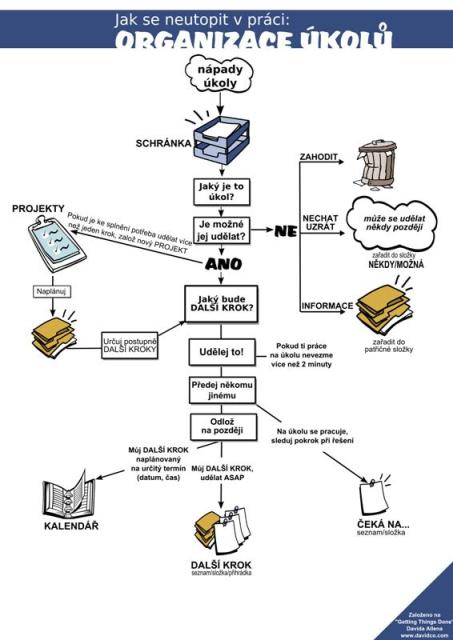
\includegraphics[width=1\textwidth]{pictures/gtd_graph}
	\caption{Digram zpracování schránky dle metodiky \GTD\cite{gtd_graph}}\label{fig:gtd_graph}
\end{figure}

Jak \GTD graf interpretovat (popíši důležité body):
\begin{enumerate}[nosep]
\item Co je to za úkol?
Potřebujeme se nad úkolem zamyslet, čeho se týká a co bude potřeba k jeho splnění. 
\item Realizovatelný/ nerealizovatelný. 
Zde se rozhodujeme, jestli úkol můžeme a chceme splnit. Nerealizovatelný úkol může být pouhá informace. Něco o čem zatím neuvažujeme a nebo pro nás není úkol relevantní a zahazujeme jej.
\item Pro realizovatelné úkoly zjistíme kolik kroků bude potřeba k jejich splnění. V případě, že jich je více zakládáme projekt a pod ním více úkolů. Hierarchie projektů a úkolů má stromovou strukturu, kde úkoly jsou vždy listy stromu.
\item Provedení úkolu
	\begin{enumerate}[nosep]
		\item trvá-li splnění úkolu kratší dobu než 2 minuty - splňme ho
		\item úkol musí vyřešit někdo jiný - deleguj ho
		\item úkol řeším a rozhodnu se o dalším kroku nebo zařadím do kalendáře
	\end{enumerate}
	Po vyhodnocení úkol končí vždy ve stavu, kdy je jasné jeho další zpracování.
\end{enumerate}
\vspace*{1\baselineskip}

Pravidelné vyprazdňování našich schránek představuje práci navíc a z počátku k němu bude existovat odpor. Musíme docílit návyku a plné důvěry, proč to děláme.

Zde už potřebujeme jednotný systém pro správu našich úkolů a projektů. Jeho navržením se budu zabývat v další kapitole.


Důležité pojmy z \GTD
\begin{itemize}
	\item \textit{Činnost/ závazek/ věc/ úkol} -- něco, co máme vykonat a k čemu jsme se zavázali
	\item \textit{Úkol} -- zde ve smyslu konkrétního kroku směřujícího ke splnění činnosti 
	\item \textit{Projekt} -- může obsahovat další \textit{projekty} a úkoly společné pro jednu činnost 
	\item \textit{Schránka} -- místo/ místa na kterých se nacházejí naše činnosti. Zpravidla se jedná o email, šanony,\dots	
\end{itemize}

\subsubsection{Pravidelná kontrola úkolů}

Kritickým klíčem k úspěchu jsou pravidelná zhodnocení všech aktuálních úkolů. Ideálně každý týden. Naším cílem je udržet si plný přehled o úkolem a zohlednit do nich současné priority.

Stejně jako u vyprazdňování schránky se snažíme o vytvoření návyku.

\subsubsection{Co mám dělat?}

Otázkou, kterou si nyní musíme zodpovědět je, jak nám náš seznam úkolů pomůže v rozhodnutí, co nyní dělat.

K tomu nám budou sloužit \textit{kontexty}.

Představme si, že máme chvíli času před schůzkou a po ruce mobilní telefon. Musíme mít možnost rychle zjistit úkoly splnitelné zavoláním z mobilního telefonu. U úkolů zavedeme kontext představující prostředek k jeho splnění. Např. mobilní telefon, notebook, internet, domov,...

Kontexty jsou pro každého z nás specifické a potřebujeme mít možnost si je spravovat.

Dalšími možnými filtry jsou \textit{dostupný čas}, \textit{dostupná energie} (jak moc \uv{svěží} musíme být jeho splnění) a \textit{priorita}.

\subsection{Shrnutí metodiky}

\begin{itemize}
	\item \textit{vše máme mimo naši mysl} --
	cokoliv potřebujeme udělat máme poznamenáno mimo naši hlavu 
	\item \textit{známe další krok}
	\item \textit{umíme naše schránky zpracovat}
	\item \textit{jednotný systém.}
	Máme jednotný systém, kam zaznamenáváme všechny úkoly/ projekty při zpracování schránky. Máme k němu 100\% důvěru a umíme ho správně použít.	
\end{itemize}


\section{Současné implementace}

\subsection{Toodledo}

Odkaz: www.toodledo.com\\
Podporovaná zařízení web: ano, iOS: ano, Android: ano

Výhody:
Plně podporuje metodiku GTD. Zakládání a editace úkolů je zde velmi snadná a vše je ukládané okamžitě při změně. U úkolů lze nastavit široké spektrum filtrů od základních kontextů až po definování lokace.
Podporuje Google Calendar (widget).

Nevýhody:
Neobsahuje integraci se sociálními sítěmi.  
Projekty jsou až od placené verze.

Tento systém v současnosti používám pro své osobní plánování.

\begin{figure}\centering
	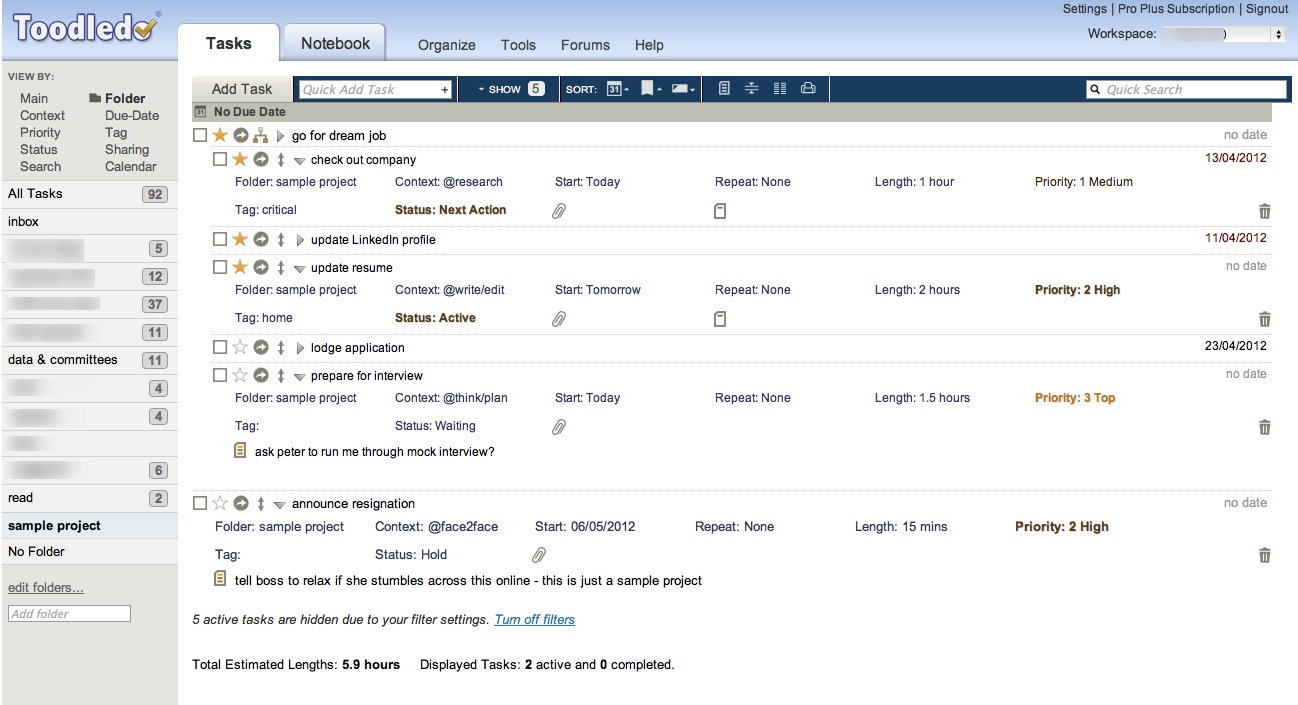
\includegraphics[width=1\textwidth]{pictures/toodledo_overview}
	\caption{Podoba webové aplikace ToodleDo.\cite{toodledo_overview}}\label{fig:toodlefo_overview}
\end{figure}

\newpage

\subsection{Doit.im}

Odkaz: doit.im\\
Podporovaná zařízení web: ano, iOS: ano, Android: ano

Výhody:
Plně podporuje metodiku GTD. Příjemná minimalistická aplikace, která je ihned po registraci připravena k použití.  

Nevýhody:
Mírně nepřehledná webová aplikace.
Podpora Google Calendar až do placené verze.

\begin{figure}[h]
	\makebox[\textwidth][c]{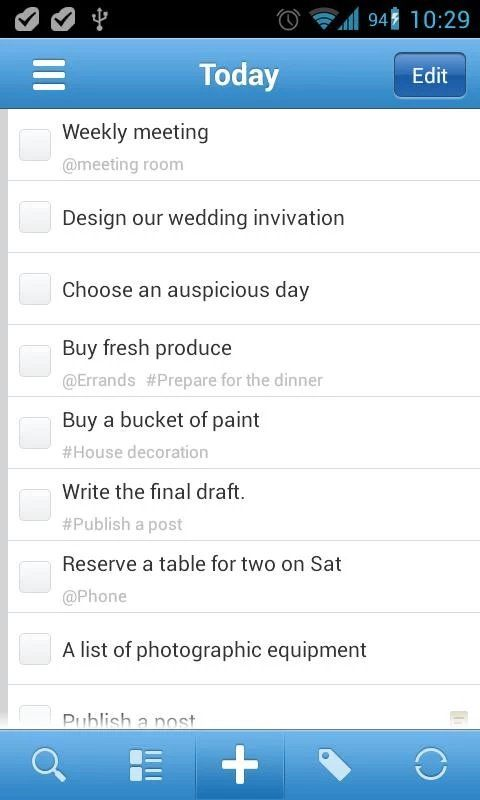
\includegraphics[height=0.7\textwidth]{pictures/doit_overview}}
	\caption{Mobilní aplikace Doit.\cite{doit_overviewgram}}\label{fig:doit_overviewgram}
\end{figure}

\newpage

\subsection{Wunderlist}

Odkaz: www.wunderlist.com\\
Podporovaná zařízení web: ano, iOS: ano, Android: ano

Výhody:
Plná podpora \GTD. Pěkné grafické zpracování s další možností přizpůsobení. Po registraci má vše potřebné k okamžitému použití. Jako u ToodleDo jsou změny okamžitě ukládány. Zakládání úkolů zasláním emailu. Sdílení úkolů.

Nevýhody:
Bez sociálních sítí. 


\begin{figure}[h]
	\makebox[\textwidth][c]{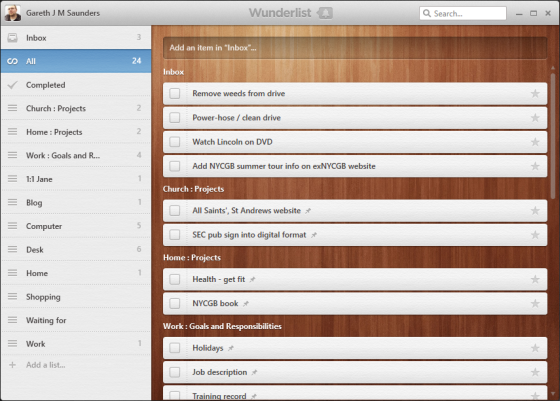
\includegraphics[height=0.7\textwidth]{pictures/wunderlist_overview}}
	\caption{Wunderlist \cite{wunderlist_overview}}\label{fig:wunderlist_overview}
\end{figure}

\newpage
	
\subsection{Todoist}

Odkaz: todoist.com\\
Podporovaná zařízení web: ano, iOS: ano, Android: ano

Výhody:
Projekty jsou zde součástí základní verzí. Pokud chceme jednoduché ovládání bez další funkcí.

Nevýhody:
Nesplňuje národy \GTD, ale umožňuje všechny potřebné základní funkce. 
Desktopová aplikace vychází z omezení mobilních zařízení a nevyužívá velkou plochu. 

\section{Shrnutí analýzy metodiky \GTD}

Z samotné metodiky \GTD jsem odvodil tyto nároky na aplikaci:
\begin{itemize}
\item \textit{Základní funkce.}
Není třeba vytvářet složité funkce. Ale ty které existující, musí být spolehlivé a uživatel nesmí mít problém s jejich ovládáním. 
\item \textit{Dostupnost.}
Aplikace se nemůže soustředit pouze na jednu platformu a musí být dostupná z více platforem (web, mobilní zařízení,...). 
\item \textit{Spolupráce s aplikacemi třetích stran.}
U uživatele lze očekávat facebook/ gmail účet a aplikace může toto využít.
\end{itemize}

Současné implementace můj závěr potvrzují. I u malých projektů je podpora pro všechny platformy téměř samozřejmostí. Minimalistické na funkčnost zaměřené uživatelské rozhraní. Synchronizace k emailovými účty je často také přítomna, ačkoliv je už součásti placené verze.

\textit{Implementace bude obsahovat}
\begin{itemize}
\item \textit{Aplikace pro centrální uložení dat vystavující \acrshort{ws} pro jejich správu}
\item \textit{Aplikace pro OS Android}
\end{itemize}

\chapter{Návrh}

Tato kapitola popisuje volbu technologií pro implementovanou aplikaci poskytující centrální uložení dat skrze \acrshort{ws} a aplikaci pro \acrshort{os} Android. Nároky na technologie vycházejí ze závěrů analýzy předešlé kapitoly a dále je rozvíjejí.
Protože jedna z aplikací potřebuje hosting, budeme hledat vhodný server splňující naše potřeby.

\section{Rozdělení aplikace}

Ze závěrů analýzy vzešlo, že aplikace musí být pro uživatele dostupná více platformách zahrnující např. mobilní zařízení a web. Proto jsem se rozhodl rozdělit návrh aplikace na dvě části. První bude zajišťovat centrální uložení dat. Druhá pak zajistí pro uživatele samotné GUI pro osobní plánování a správu dat deleguje na první aplikaci. Díky tomuto návrhu se zbavím nutnosti implementovat uložení dat na každé uživatelské aplikaci.

\subsection{Aplikace pro centrální uložení dat}

Skrze \acrshort{ws} bude poskytovat centrální uložení dat do databáze. Služby budou dostupné přes internet a samotná aplikace bude nasazena do aplikačního serveru.

\subsection{Mobilní aplikace pro Android}

První implementace GUI cílená na mobilní zařízení se systémem Android. Fungovat bude na  principu tenkého klienta\cite{gtd_thin_client}.

\section{Model nasazení}

\begin{figure}[h!]\centering
	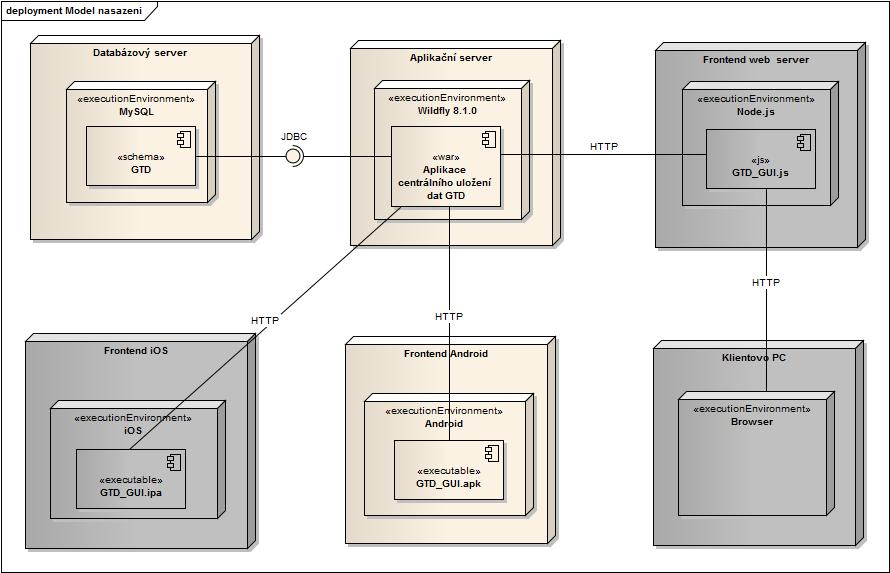
\includegraphics[width=1\textwidth]{pictures/gtd_deployment_model}
	\caption{Model nasazení GTD (šedivě zbarvená nasazení ukazují úvahy dalšího rozšíření)})\label{fig:gtd_deployment_model}s
\end{figure}

\todo{Komentář, že se jedná o navazující projekt z SP2}
Vycházení z návrhu rozdělení aplikace. GUI aplikace jsou unikátní pro každou platformu s centrální aplikací pro správu data komunikují přes HTTP protokol.

\section{Technologie}

\subsection{Aplikace pro centrální uložení dat}
  
\subsubsection{Webová služba -- \acrshort{rest} \acrshort{api}}

Při volbě webového \acrshort{api} jsem se rozhodoval mezi dvěma typy webových služeb.
\newline
\begin{itemize}
	\item \textit{SOAP}
	\item \textit{REST}
\end{itemize}
\vspace*{1\baselineskip}

Nyní se soustředím na hlavní rozdíly mezi těmito službami.

\begin{table}\centering
\caption{Rozdíly mezi SOAP a REST}\label{tab:ws_compare}
\begin{tabular}{|p{3cm}|p{3cm}|p{5.5cm}|}\hline
Typ		& SOAP		& REST \tabularnewline \hline \hline
Format dat\cite{ws_compare_swati}		& XML		& nezávislý (XML, JSON, plain) \tabularnewline \hline
Protokol\cite{ws_compare_swati}		& více možných (HTTP, SMTP,..)		& HTTP \tabularnewline \hline
Možnost cachování\cite{ws_compare_swati}		& ne		& ano \tabularnewline \hline	
Formát specifikace\cite{ws_compare_table}\cite{ws_compare_soapui} & WSDL\cite{ws_soap_wsdl}	& existují formáty jako \acrshort{wadl}\cite{ws_wadl}, Swagger\cite{ws_swagger}, \acrshort{raml}\cite{ws_raml} a další, ale žádný nemůžeme považovat na hlavní \cite{ws_comparison} \tabularnewline \hline 		 
Vystavuje\cite{ws_compare_steve}		& operace & zdroje \tabularnewline \hline
Zabezpečení\cite{ws_compare_steve}		& SSL + WS-Security & SSL \tabularnewline \hline  
Rozšířenost\cite{ws_compare_steve}		& \multicolumn{2}{p{8.5cm}|}{REST získává na stále větší popularitě . Příkladem uvedu např. Google, který se nahradil své dřívější SOAP API právě RESTem.}  \tabularnewline \hline 
Rychlost zpracování\cite{ws_compare_armel} 	& \multicolumn{2}{p{8.5cm}|}{XML parsing je pomalejší než JSON}  \tabularnewline \hline 	 		  		
Jednodušší implementace\cite{ws_compare_swati}		&\multicolumn{2}{p{8.5cm}|}{u RESTu na straně klienta i serveru} \tabularnewline \hline 	 				
\end{tabular}
\end{table}

Návrh nepočítá s využitím zabezpečení (přihlášení bude řešeno pomocí tokenu \todo{link na zabezpeceni})  a komunikace bude probíhat přes HTTP protokol (SOAP ztrácí výhodu).
Myšlenkou RESTu je poskytnout CRUD\cite{ws_compare_steve} operace nad vystavenými zdroji\cite{ws_crud} a to přesně odpovídá potřebám navrhovaného centrální uložení dat.  Další výhody jako rychlá implementace a přenos dat ve formátu JSON je podpořily volbu. 

Volba pro \acrshort{ws} je REST.

\label{ws_compare_mulesoft}
Pro návrh REST API bude použit jazyk \acrshort{raml}. Jedná se nový jazyk založení na formátu \acrshort{yaml}, který v říjnu 2014 přešel do verze 1.0\cite{ws_raml} a na jehož vývoji se podílí technologičtí odborníci ze známých IT firem\cite{ws_raml_wiki}. Díky \acrshort{yaml} se kód dobře píše a výsledný dokumentace je čitelná. Pro vývoj bude použito webového prostředí od firmy MuleSoft\cite{ws_raml_mulesoft}. Jedná se o firmu, která se na \acrshort{raml} úzce propojena, protože na specifikaci \acrshort{raml} se  podílí její CTO\footnote{www.linkedin.com/in/sarid}.
\vspace*{1\baselineskip}

\todo{tabulka rest api}

\subsubsection{Programovací jazyk -- Java}

Volba programovacího jazyka byla pro mě jasná: \textit{Java}.

Pro vývoj aplikace jako webové služby založené na RESTovém API můžeme využít celou škálu programovacích jazyků. Od nejběžnějšího PHP/ Python/ ASP, přes Javu k méně známým jako Ruby a další\dots

Java je perspektivní, velice rozšířený a univerzální jazyk s rozsáhlou komunitou. Komunita, velké množství frameworků a další rozšíření dělají z Javy, tak silný programovací jazyk, kterým bezesporu je.  

Přesto má volba pro Javu vzešla hlavně z mého zaměstnání a potřeby se v tomto programovacím jazyce zdokonalit. 

\subsubsection{Základní framework -- Spring}

Nyní hledám framework, který mi umožní rychle implementovat REST API. Ve světě Javy na podobné otázky existuje vždy více možných odpovědí. 
Podívejme se na hlavní možnosti:
\begin{itemize}
	\item \textit{JAX-RS\footnote{jax-rs-spec.java.net}} -- REST API od Javy
    \item \textit{Jersey\footnote{jersey.java.net}} -- implementace REST API založená na JAX-RS
    \item \textit{Spring MVC\footnote{http://docs.spring.io/spring/docs/current/spring-framework-reference/html/mvc.html}} -- vlastní implementace z rodiny Spring
\end{itemize}

Všechny řešení podobný postup. Pomocí anotací ovlivňují chování tříd a method pro příjem/ odeslání zpráv v kontextu REST API. 

Rozhodl jsem se pro Spring. Hlavním důvodem byl rozsah celého Spring frameworku. Díky jeho univerzálnosti, snadné konfigurovatelnosti a dobré dokumentaci je použití Springu a Javy téměř standardem.    

Méně častou volbou je mé rozhodnutí pro rozšíření Spring boot\footnote{projects.spring.io/spring-boot/}. Slouží pro vytváření stand-alone Spring aplikací a zlehčuje základní konfiguraci aplikace. Pozitivním efektem je také odstranění \acrshort{xml} konfigurací.

\subsubsection{Persistence dat -- Hibernate}
\label{technology:hibernate}
Pro persistenci dat jsem zvolil framework Hibernate\footnote{hibernate.org}. 

Používá \acrshort{orm}, což je způsob, kdy je objektový model mapován na relační databázi. Programátor pomocí anotací (nejčastěji nad třídami modelu) definuje podobu databázových objektů, ale o samotnou správu na úrovni databáze se už nestará. Hibernate také zajišťuje nezávislost na použité databázi. Nicméně např. pro Oracle databázi je potřeba použít speciálních anotací (databáze nemá auto inkrementální sloupce a pracuje přes definici sekvencí hodnot).

Použití Hibernate je Springem přímo podporováno a jeho konfigurace je velice snadná.

\subsubsection {Databáze -- MySQL}

Jako databázi jsem si zvolil MySQL. 

Jedná se o relační databázi, která si v současnosti získává obrovskou oblibu. Je to díky její nenáročnosti, jednoduchosti, výkonnosti a stabilitě. Vlastníkem je firma Oracle, vydávající také databázi Oracle DB, která už vyžaduje specializovanou správu a není pro tento projekt vhodná. Pro administraci databáze jsem zvolil phpMyAdmin. A to díky mým dřívějším zkušenostem s jeho používáním.  

\subsubsection {Aplikační server Wild Fly}

Jako aplikační server jsem zvolil WildFly\footnote{wildfly.org} ve verzi 8.2.\newline

Jedná se pokračování známého JBoss AS\cite{wildfly}.\newline

\textit{Potřebné vlastnosti} 
\begin{itemize}[nosep]
	\item \textit{rychlá instalace}
	\item \textit{funkce auto deploy} -- zkopírování waru\footnote{http://docs.oracle.com/javaee/6/tutorial/doc/bnaby.html} aplikace do určité složky serveru dojde k jejímu automatickému nasazení
	\item \textit{administrátorské rozhraní}
	\item \textit{dokumentace} -- díky jeho rozšíření existuje velké množství návodů  
	\item \textit{podpora Java EE\footnote{http://www.oracle.com/technetwork/java/javaee/overview/index.html}}
\end{itemize}

\subsubsection{Hosting - DigitalOcean}

Pro hosting jsem zvolil služby DigitalOcean\footnote{www.digitalocean.com}.

Jako další možnost byl server OpenShift\footnote{www.openshift.com}. Ten poskytuje pevně dané aplikace, které je možné na virtuální server nainstalovat. Instalace serveru probíhá formou konfigurace a je díku tomu velmi snadná. Bohužel omezení systémových prostředků u neplacené verze vedlo k nespolehlivosti mého serveru a hledání jiné varianty. 

DigitalOcean poskytuje tzv. droplet. Funguje jako virtuální server a správce si volí \acrshort{os}, který je něm automaticky nainstalován. Další instalace se už provádějí přímo ve vybraném \acrshort{os}. Mou volbou byl Ubuntu verze 14. Jde jednoduchý a spolehlivý linuxový systém se kterým mám jen kladné zkušenosti. 

DigitalOcean je placený, ale v rámci GitHub Education packu\footnote{education.github.com/pack} je pro studenty k dispozici 100 dolarový kapitál. To stačí na mnohaměsíční provoz i silnějších variant dropletů s více systémových prostředků. Pro naši aplikaci jsem zvolil variantu 2 GB paměti, 2 CPU, 40 GB SSD disk za 20 dolarů na měsíc.  


\subsection{Mobilní aplikace pro Android}

\subsubsection {OS Android}

Rozhodl jsem se svou mobilní aplikaci implementovat pro \acrshort{os} Android.

Vybíral jsem mezi \acrshort{os} Android do firmy Google\footnote{www.android.com} a iOS od firmy Apple\footnote{www.apple.com/cz/ios/}.
 
Celkové množství aplikací je u obou \acrshort{os} téměř stejné a ani náročnost vývoje neznamená výrazné rozdíly.\cite{android_what_choose}. Rozdíl programovacích jazyků (Android:Java a iOS:Objective-C) pro mě znamená důležitý faktor. U předešlé aplikace jsem se rozhodl pro Javu a díky Androidu mohu zůstat ve stejném programovacím jazyce.

\textit{Trh}
Android má silnou převahu v zastoupení na světovém trhu. Zatímco iOS si drží 15\% podíl, Android se pohybuje na 80\% \cite{android_market}. Silnější pozice dosahuje iOS na trhu v U.S., kde můžeme zastoupení obou \acrshort{os} považovat za vyrovnané \cite{android_market_us}. 
Pro mě je důležité, že Android při stejném množství aplikace poskytuje širší uživatelskou základnu. 

Závěrem analýzy existujících implementací osobního plánování je důraz na podporu co nejširšího spektra platforem. Z tohoto pohledu chápu mé rozhodnutí pro vývoj na \acrshort{os} Android jako volbu první mobilní platformy pro implementaci. A v rámci další rozvoje projektu plánuji podporuji pro další.\newline

\textit{Shrnutí}
\begin{itemize}[nosep]
	\item \textit{Java} -- mohu stavět na současných znalostech tohoto jazyka a využít stejné vývojové prostředí
	\item \textit{zastoupení na trhu} -- více uživatelů mi dává vyšší šance si najít své zákazníky
	\item \textit{osobní preference} -- vlastním mobil s \acrshort{os} Android
\end{itemize}

\subsubsection{Android-bootstrap}
\label{technologie:androdi:boostrap}
Pro implementaci jsem se rozhodl použít framework Android-bootstrap od Donna Felkera \footnote{http://www.androidbootstrap.com/}.

Framework dodává implementaci základních funkcí aplikace pro \acrshort{os} Android. Používá se jako základ při vytváření aplikace a umožňuje rychlý vývoj. Zdrojové kódy jsou přístupné na GitHubu, a autor se společně s komunitou podílejí na dalším rozvoji.\newline

\textit{Obsahuje}
\begin{itemize}[nosep]
	\item \textit{napojení na REST API}
	\item \textit{implementace přihlašování}  
	\item \textit{stránkování jako hlavní komponenta uživatelského rozhraní} -- snadné rozšíření o další stránky
	\item \textit{vlastní implementace zobrazení seznamu dat} -- načtení dat v asychronním vlákně, specifikace zobrazení pomocí vlastního layoutu\footnote{http://developer.android.com/guide/topics/ui/declaring-layout.html}  
	\item \textit{jednotný grafický vzhled}	
\end{itemize}

Nevýhodou je nárok na verzi Android \acrshort{sdk} 15 a vyšší.


\subsubsection {Verze SDK Android}

Rozhodl jsem pro minimální verzi \acrshort{sdk} 16 (Android verze 4.1 s označením Jelly bean) a cílovou verzi \acrshort{sdk} 19 (Android verze 4.4 s označením Kitkat).
Toto rozhodnutí vzešlo z nároků mnou zvolené technologie a současného stavu trhu.

Použitím frameworku Bootstrap (viz \ref{technologie:androdi:boostrap}) jsem stanovil minimální verzi \acrshort{sdk} na 15 a vyšší. V rámci vývoje jsem následně použil funkce vyžadující verzi \acrshort{sdk} 16+.

Autoři Androidu doporučují volbou \acrshort{sdk} pokrýt 90\% aktivních zařízení\cite{android_sdk_recommendation}. V aktuálním zastoupení \acrshort{sdk} vede verze 19 a suma od verze 4.1 výše je cca 88\%\cite{android_sdk_graph}. 

\subsubsection{Facebook}
\todo{Facebook}

\subsubsection{Google}
\todo{Google navrh}

\chapter{Návrh}

Tato kapitola se zaměřuje na definování základních charakteristik aplikace. Najdete zde návrh specifikace REST API a webového vývojového prostředí od společnosti Mulesoft, které je k návrhu použito. 

Kapitola dále popisuje použitý datovým model.

Nakonec se seznámíte s postupem pro propojení mobilní aplikace na Facebook a Google kalendář. Přidělíme každé aplikaci oddělené úkoly. Mobilní aplikace zajistí přihlášení uživatele a získání access tokenu. Tento token předáme aplikaci pro centrální uložení dat a ta zajistí samotnou práci s API protistrany.

\section{REST API}
\label{rest_api_design}

Budeme pracovat s těmito čtyřmi metodami HTTP \ref{tab:RESTfulAPI_definice}:

\begin{table}[!h]\centering
\caption{Funkce HTTP method}\label{tab:RESTfulAPI_definice}
	\begin{tabular}{l c}
		\toprule
		\textbf{HTTP metoda} & \textbf{Popis} \\ \midrule \midrule
		GET & získá informace daného zdroje  \\ \midrule	
		POST & vytvoří nový zdroj\\ \midrule
		PUT & aktualizuje daný zdroj  \\ \midrule
		DELETE & smaže daný zdroj \\ \bottomrule
	\end{tabular}
\end{table}

Navržené REST API rozhraní je zobrazeno v tabulkách \ref{tab:RESTfulAPI_rozhrani_s} a \ref{tab:RESTfulAPI_rozhrani_s} (* -- představuje společnou URL adresu určenou nasazením a verzí API).

\begin{table}\centering
\caption{Rozhraní REST API přístupné s tokenem}\label{tab:RESTfulAPI_rozhrani_s}
	\begin{tabular}[t]{l l c}
		\toprule
		\textbf{Zdroj URI} & \textbf{HTTP metoda}\\ \midrule \midrule
		1&*/projects/ & POST \\ \midrule
		2&*/projects/ & GET \\ \midrule
		3&*/projects/\{id\} & GET \\ \midrule
		4&*/projects/\{id\} & PUT \\ \midrule
		5&*/projects/\{id\} & DELETE \\ \midrule  
		6&*/tasks/ & POST \\ \midrule
		7&*/tasks/ & GET \\ \midrule
		8&*/tasks/\{id\} & GET \\ \midrule
		9&*/tasks/\{id\} & PUT \\ \midrule
		10&*/tasks/\{id\} & DELETE \\ \midrule       
		11&*/tasks/\{id\}/facebookPublish & POST \\ \midrule
		12&*/tasks/\{id\}/googlePublish & POST \\ \midrule
		13&*/persons/ & GET \\ \midrule
		14&*/persons/\{id\} & GET \\ \midrule
		15&*/persons/\{id\} & PUT \\ \midrule
		16&*/persons/\{id\} & DELETE \\ \midrule  	
		17&*/persons/auth & GET \\ \midrule  				
	\end{tabular}
\end{table}

\begin{table}\centering
	\caption{Rozhraní REST API přístupné bez tokenu}\label{tab:RESTfulAPI_rozhrani_bez}
	\begin{tabular}{l c}
		\toprule
		\textbf{Zdroj URI} & \textbf{HTTP metoda}\\ \midrule \midrule
		*/authenticate/\{userLogin\} & GET \\ \midrule
		*/persons & POST \\ \midrule
	\end{tabular}
\end{table}


Na základě volby v \ref{ws_compare_mulesoft} vznikl návrh REST API ve webovém vývojovém prostředí Mulesoft.\newline 

\begin{tabular}{l l}
	Přístupné přes:&\href{''https://anypoint.mulesoft.com/#/signin''}{Mulesoft API Designer}\\
	Příhlašovací jmeno:&drugnanov\\
	Heslo:&Qazwsxedc369\\
\end{tabular}

\begin{figure}[h!]\centering
	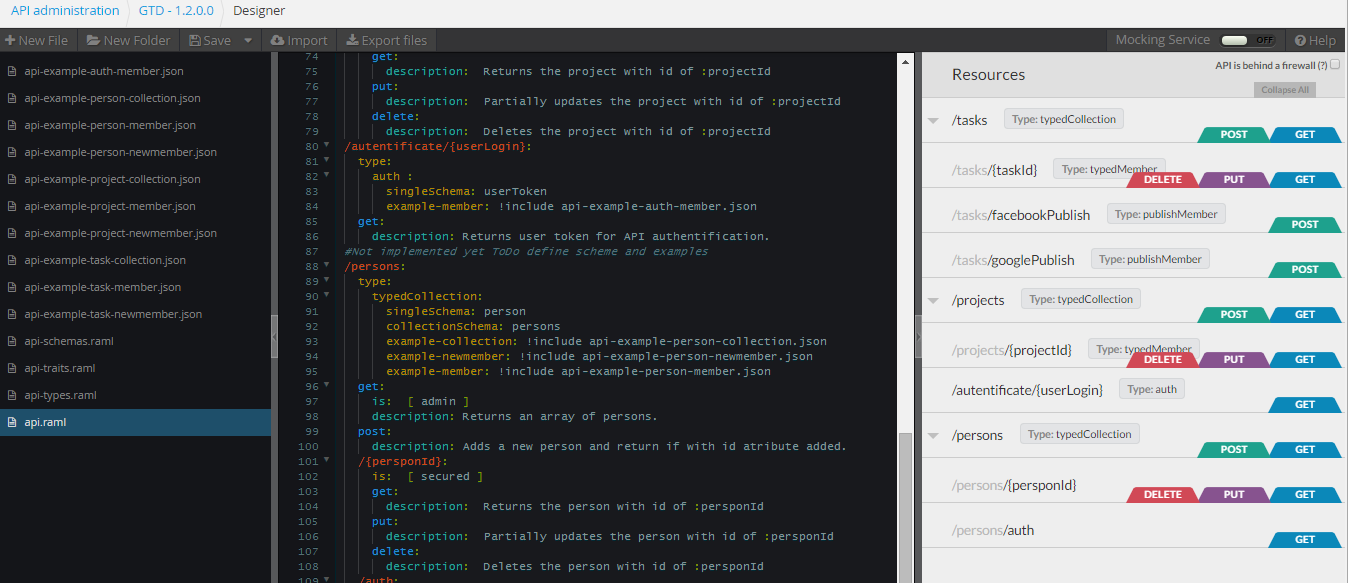
\includegraphics[width=1\textwidth]{pictures/gtd_raml_anypoint}
	\caption{Webové prostředí pro návrh REST API ve specifikaci RAML od firmy Mulesoft}\label{fig:gtd_raml_ide}
\end{figure}

Práce s tímto prostředím je příjemná. Některé funkce potřebují ještě vylepšit. Chybí inline nápověda v kontextu specifikace RAML a např. auto complete nepracuje s objekty vytvořenými uživatelem. Zároveň příkladů návrhu API v jazyku RAML na webu není mnoho. To bohužel prodlužuje čas učení a samotného návrhu. Přesto má tento nástroj vykročeno stát se součásti DDD\cite{ws_raml_ddd}. 

\section{Databázový model}
\label{design:database_model}
V \ref{technology:hibernate} jsem se rozhodli pro použití Hibernatu. To nám umožňuje specifikovat strukturu databáze přímo v datovém modelu aplikace. Specifikace se provádí pomocí anotací nad objekty tříd, metod a atributů\cite{design_hibernate_annotations}. 


\chapter{Realizace}

V této kapitole se seznámíme s praktickým použitím dříve zvolených technologií. U aplikace pro centrální uložení dat si ukážeme strukturu projektu, podobu práce s REST API, generování struktury databáze pomocí hibernatu, identifikace uživatele s použitím tokenu a práci s API Facebooku a Google kalendáře.
U android aplikace si uk\todo{co s ukážeme u android aplikace}
\newpage

\subsection{Aplikace pro centrální uložení dat}

Zde si ukážeme části implementace aplikace pro centrální uložení dat.

\subsubsection{Struktura projektu}
 
\begin{figure}[h!]
\dirtree{%
.1 libs\DTcomment{externi knihovny používané aplikací}.
.1 src\DTcomment{základní balík implementace projektu}.
.2 main\DTcomment{balík aplikace}.
.3 java\DTcomment{složka s kódy aplikace}.
.4 GTD\DTcomment{základní balík GTD}.
.5 BL\DTcomment{balík buisiness vrstvy}.
.5 DL\DTcomment{balík datové vrstvy}.
.5 restapi\DTcomment{balík pro REST API}.
.3 resources\DTcomment{složka obsahující konfigurace}.
.4 database\DTcomment{složka obsahující pomocné skripty pro správu databáze}.
.4 messages\DTcomment{složka pro stringové konstanty aplikace}.
.4 gtd.api.properties\DTcomment{property aplikace}.
.4 hibernate.cfg.xml\DTcomment{konfigurace hibernatu}.
.4 logback.xml\DTcomment{konfigurace logování pomocí logbacku}.
.2 test\DTcomment{složka obsahující unit testy}.
.1 build.gradle\DTcomment{build soubor pro Gradle}.
.1 settings.gradle\DTcomment{nastavení Gradlu}.
}
\end{figure}

\subsubsection{REST API}

ukázka kontroleru

odchycení výjímek

ukázka servisy pro obsluhu volání (např add person)
\subsubsection{Databáze}

Příklad použití anotací na základě \ref{realization:hibernate_example}.

\lstinputlisting[label=realization:hibernate_example,caption=Příklad použití Hiberante]{codes/hibernate_person.java}

Význam anotací dle \cite{design_hibernate_annotations}.

Doplněním anotací k prvkům datového modelu a konfigurací hibernatu byla v MySQL vygenerována následující databázová struktura \ref{fig:gtd_database_model}.

\begin{figure}
	\makebox[\textwidth][c]{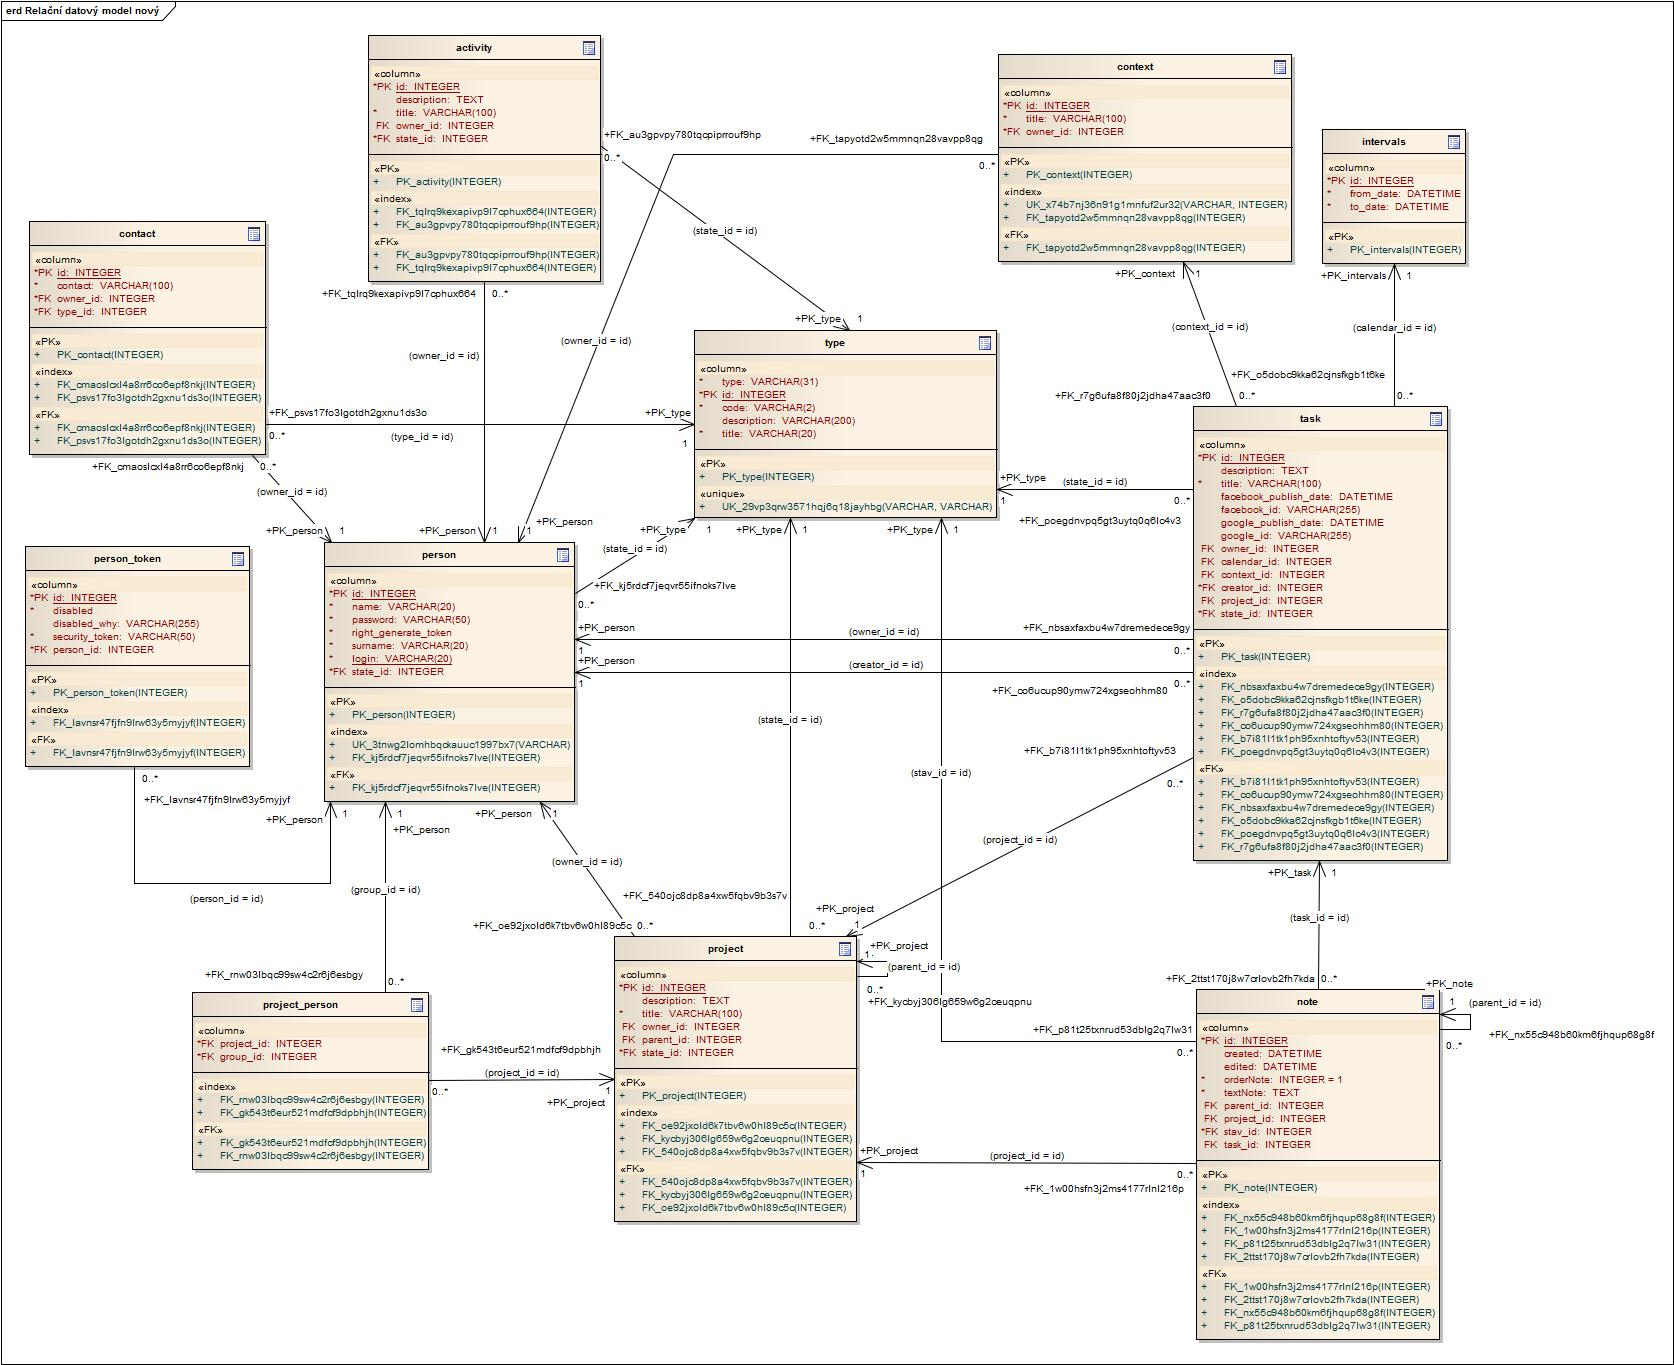
\includegraphics[height=1.17\textwidth, angle=90]{pictures/gtd_entity_relationship_diagram}}
	\caption{Databázový model}\label{fig:gtd_database_model}
\end{figure}


\subsubsection{Identifikace uživatele}

Identifikace uživatele je realizována formou tokenu v hlavičce HTTP požadavku. Token lze získat pomocí dvou způsobů (viz. \ref{tab:RESTfulAPI_rozhrani_bez}):
\begin{itemize}[nosep]
	\item \textit{registrací} -- po vytvoření účtu je ve vráceném objektu \textit{osoby} obsažen také token
	\item \textit{přihlášení} -- autentifikace pomocí loginu a hesla uživatele, v takovém případě je zpět vrácen pouze token a login uživatele.
\end{itemize}

Při vytvoření uživatele je token vygenerován automaticky. V případě přihlášení je vrácen aktivní token uživatele. Pokud uživatel token nemá (např. token byl deaktivován) a má právo si token vytvořit, je mu automaticky vygenerován.

Pokud uživatel už aktivní token má, může použít dotaz číslo 17 z \ref{RESTfulAPI_rozhrani_s}. API na základě tokenu rozpozná \textit{osobu} a vrátí její objekt \textit{osoby} obsahující všechny tokeny. 

Token je generován pomocí kódu v \ref{api_token_generated} (person je objekt typu Person).

\begin{lstlisting}[label=api_token_generated,caption=Generování uživatelského tokenu]
	String stringToCrypt = person.toString() + PersonToken.tokenSalt + currentTimeMillis();
	String hash = HashConverter.md5(stringToCrypt);
\end{lstlisting}



\subsubsection{Facebook}

práce s access tokenem

vypublikování tasku na zeď uživatele

\subsubsection{Google}

práce s access tokenem

vypublickování tasku do google kalendáře


\subsection{Mobilní aplikace pro Android}

\subsubsection{Rozložení projektu}

--složky a k čemu slouží

\subsubsection{Konzumace REST API}

-- konzumace rest api

\subsubsection{Asynchronní načítání dat}

--ukázka takového volání 

--jak se při získání/ nezískání výsledku

--Bus listenery

\subsubsection{Facebook}

-- jak zalozi aplikaci na facebooku a spravne ji nastavit

-- nastaveneni projektu

-- ziskani access tokenu přihlášením uživatele 

\subsubsection{Google}

-- jak zalozi aplikaci na facebooku a spravne ji nastavit

-- nastaveneni projektu

-- ziskani access tokenu přihlášením uživatele 

\section{Hosting}

--postup instalace 

--správa

\section{GitHub}

--zpřístupnění kódu na GitHubu ano?

\todo{AnyPoint}

\todo{Program pro převod JSON do objedků  d:01.Skola01.Bakalarka30.Vyvoj BP GTD GeneratorPOJOs}

\subsection{title}

\section{Návrhy k rozvoji}
Apple aplikace 
Testování na reaálných zařízeních a úprava kódu aby to fungovalo

refactoring Hibernate


Fungování s email načtením

\begin{conclusion}

Metodika \GTD do mého života přinesla nový směr a podle něj se snažím řídit. Mysl potřebujeme použít k řešení problému a ne jako diář, který ještě funguje velmi podivně a události nám připomíná velmi nahodile. Diář si musíme vytvořit mimo ni. Na internetu nám k tomu pomůže celá řada produktů. Je jen na nás, který si vybereme. A volba je důležitá. Protože metodika nás nabádá, že musíme mít naprostou důvěru ke spolehlivosti svého systému a používat ho rádi. Plánování a revize úkolů se musí stát pravidelnou činností.

Mnou navržený systém se ukázal jako vhodný.

Framework Spring, který jsem použil pro aplikaci poskytující centrální uložení dat, mi pomohl k vytvoření dobře škálovatelné a udržovatelné aplikace. Vybrané REST API dostálo mým předpokladům, pro které jsem ho vybral. Implementace není náročná na straně serveru ani klienta a plně vyhovuje potřebám aplikace. Stejně tak má volba Hibernatu pro \acrshort{orm} řešení mě dobře odstínila od databázového prostředí. Zde se ukazuje síla anotací. Pomocí nich lze provádět širokou škálu konfigurací bez nutnosti externích konfiguračních souborů. Proto jsem pomocí anotací konfiguroval  samotnou aplikaci a zde mi práci ulehčil vybraný Spring Boot. 

Pro hosting jsem zvolil server Digiocean. Zde jsem vytvořil vlastní Linux server, nainstaloval a nakonfiguroval aplikační server WildFly a databázi MySQL s phpAdminem a nasadil REST API aplikaci.

Mobilní aplikaci jsem vyvinul a testoval na lokálním emulátoru Genymotion s instalovanou verzí Androidu 19. Volba Bootstrapu byla výborná a pro účely mé aplikace plně vyhovující. Framework poskytuje dostačující infrastrukturu a zároveň je sám založen na další knihovnách usnadňujících vývoj. 

Nastudoval jsem specifikace API Facebooku a Google kalendáře. Umožňuji uživateli publikovat úkol na jeho vlastní zeď Facebooku. Stejně může publikovat úkol do Google kalendáře. Zde jsem správně navrhl oddělit funkci publikování na dvě části a to získání přístupových práv a samotné publikování. Přístupová práva získává Android aplikace a k tomu využívá komponenty přímo od Facebooku a Googlu. Správně jsem analyzoval, že proces nelze automatizovat, ale vytvořením přístupového tokenu lze následné publikování delegovat na jinou aplikaci. O samotné publikování se stará REST API aplikace.

Práce s API Facebook i Googlu pro mě znamenala cennou zkušenost a vidím v něm velký potenciál dalšího rozvoje. V moderním internetovém prostředí už nemůže aplikace existovat izolovaně, ale je třeba ji integrovat do existujícího prostředí. A tato integrace nemá být pouze pasivní, ale také aktivní.

\todo{na čem je nasazeno, kolik lidí to používá a další rozvoj}
    



  
%Spíše vývoj v HTML 5
%
%Obecně konkurence je vysoká a prosadit se s vlastním produktem je těžké. Sám o sobě nepřináší změnu, ale spíš vlastní pohled.
%Uživatel naopak bude postrádat ultra super funkce.
%
%Zkušenost s vývojem WS a Andoridu a napojením na Facebook a Google mi poskytlo dost zkušenost a mohu použít dále ve svém profesním životě. V případě Springu a Hibernate jsem tak už učinil. 
%
%Aplikaci jsem se rozhodl dále nerozvíjet.
%
%Další otázkou je vývoj v HTML 5 jako univerzální implementace fungujícího napříč různými OS.
%
%Náročnost vývoje - v momentě, kdy potřebuji na lokálním prostředí mít spuštěno více instance IDE, lokální aplikační a databázový server a hlavně emulátor androidu. dochází k přetížení systému. 4 jádrový Intel Core i5 2,6GHz 8GB paměti.
%obrázek.

\end{conclusion}

\bibliographystyle{csn690}
\bibliography{mybibliographyfile}

\appendix

\chapter{Seznam použitých zkratek}
\printglossaries


\chapter{Obsah přiloženého CD}

%upravte podle skutecnosti

\begin{figure}
	\dirtree{%
		.1 readme.txt\DTcomment{stručný popis obsahu CD}.
		.1 exe\DTcomment{adresář se spustitelnou formou implementace}.
		.1 src.
		.2 impl\DTcomment{zdrojové kódy implementace}.
		.2 thesis\DTcomment{zdrojová forma práce ve formátu \LaTeX{}}.
		.1 text\DTcomment{text práce}.
		.2 thesis.pdf\DTcomment{text práce ve formátu PDF}.
		.2 thesis.ps\DTcomment{text práce ve formátu PS}.
	}
\end{figure}

\end{document}
